\documentclass{beamer}
\mode<presentation>
{
  \usetheme[sidebar=0,sidebarskip=2]{}
  \setbeamercovered{transparent}
}
\pgfdeclareimage[height=0.5cm]{university-logo}{unilogo2.png}
\logo{\pgfuseimage{university-logo}}

\usepackage{mathrsfs}
\usetheme{Warsaw}
\definecolor{PittBlue}{RGB}{238,36,86}
\usecolortheme[named=PittBlue]{structure}
\usepackage{amsmath}
\usepackage{amsfonts}
\usepackage{subfigure}
\usepackage{xcolor}
\usepackage{beamerthemesplit}
\usepackage{amsmath}
\usepackage{amsfonts}
\usepackage{subfigure}
\usepackage{xcolor}
\usepackage{caption}
\usepackage{mdwlist}
\usepackage{pgf,pgfarrows,pgfnodes}
\usepackage{helvet}
\usefonttheme{structurebold}

\setbeamertemplate{navigation symbols}{}
\setbeamertemplate{footline}{}
\definecolor{myblue}{RGB}{0,20,70}
\definecolor{myred}{RGB}{70,0,0}
\definecolor{mypurple}{RGB}{102,0,204}
\definecolor{mygold}{RGB}{197,179,88}
\definecolor{mygreen}{RGB}{0,128,0}
\definecolor{myorange}{RGB}{255,204,0}
\definecolor{mydarkorange}{RGB}{252,108,0}
\setbeamercolor{title}{fg=white}
\setbeamercolor{frametitle}{fg=white,bg=PittBlue}
\setbeamercolor{boxesroundedtitle}{fg=white,bg=white}
\setbeamercolor{item projected}{fg=white,bg=white}
\captionsetup{labelformat=empty,labelsep=none}
\def\Tiny{\fontsize{6pt}{6pt}\selectfont}
\renewcommand{\captionfont}{\Tiny}
\def\MediumFont{\fontsize{7pt}{7pt}\selectfont}
\usepackage [autostyle, english = american]{csquotes}
\MakeOuterQuote{"}
\usepackage{hyperref}
\usepackage{wrapfig}

\DeclareMathOperator{\Vol}{Vol}
\DeclareMathOperator{\Int}{int}
\DeclareMathOperator{\Conv}{Conv}
\DeclareMathOperator{\Area}{Area}
\newcommand{\rom}[1]{\uppercase\expandafter{\romannumeral #1\relax}}
\newtheorem{proposition}[equation]{Proposition}
\newcommand{\defv}[1]{\textbf{\textit{#1}}}

\def\definitionautorefname{Definition}
\def\theoremautorefname{Theorem}
\def\conjectureautorefname{Conjecture}
\def\lemmaautorefname{Lemma}
\def\corollaryautorefname{Corollary}
\def\remarkautorefname{Remark}
\def\propositionautorefname{Proposition}
\def\exampleautorefname{Example}
\def\assumptionsautorefname{Assumptions}

\newtheorem{assumptions}{Assumptions}[section]
\newtheorem{defs}{Definitions}[section]


\DeclareMathOperator{\spanv}{span}
\newtheorem{remark}[equation]{Remark}
\theoremstyle{definition}
\newtheorem{idea}[equation]{Idea}
\newtheorem{exampl}[equation]{Example}

\newcommand{\defvv}[1]{\textbf{\textit{#1}}}


\setbeamertemplate{itemize subitem}{\rule{4px}{4px}}
\useoutertheme{infolines}

\makeatletter
\def\blfootnote{\xdef\@thefnmark{}\@footnotetext}
\makeatother


\title[]{A WORK-IN-PROGRESS CHAT
}
\author[W\"oden Kusner TU Graz]{\\ \textbf{W\"oden Kusner}\thanks{\tiny{Supported by an FWF special research program, NSF grant 1104102 and a fellowship from the University of Pittsburgh.}}\\
Technische Universit\"at Graz\\
\raisebox{-35pt}{
\includegraphics[width=1.5in]{unilogo2.png}}
}

\date[]{\small January 2015}

\begin{document}

\frame{\titlepage}

\frame
{
\frametitle{Abstract}
Right now, one of my projects is focused on exploring the quality of measure on spheres.  We'll look at the implementation of an algorithm for computing discrepancy, some of the analysis of a problem related to the quality of a distribution of points in the compact setting, and some of the open problems that go with them.
}

%%%%%%%%%%%%%%%%%%%%%%%%%


\frame
{
\frametitle{Discrepancy}

You are probably familiar with discrepancy as a function $D:\mathbb{N}\times \mathbb{I}^\mathbb{N}\rightarrow \mathbb{I}$ measures the irregularity of the distribution of a sequence $\{x_i\}$ when truncated at a natural number
\[
D_N(\{x_i\}) = \sup_{0 \le a < b \le 1} |\frac{\#( \{x_i\}_{i\le N)} \cap [a,b]}{N} - (b-a)|.
\]

This notion can be generalized in many ways to other spaces, for example, by identifying the end points of the interval and including all connected subsets containing the point $\{0=1\}$ gives a discrepancy for a sequence of points on $\mathbb{S}^1$, the spherical cap discrepancy.  

}

%%%%%%%%%%%%%%%%%%%%%%%%%

\frame
{
\frametitle{Discrepancy}

In general, given an geometric sphere  $\mathbb{S}^{d}$ with radius 1 and normalized uniform measure $\sigma$ and an (open) spherical cap $C$ embedded in $\mathbb{R}^{d+1}$, the \emph{ local spherical cap discrepancy} of a set $X_N$ of $N$ distinct points in the $d$-sphere is given by
\[
\operatorname{D}_C[X_N] := |[\operatorname{Vol}(C) - \frac{1}{N}\# |X_N \cap C| ]|
\]
which may be viewed as a normalized difference between the expected number of points in a cap of Vol($C$) and the number of points found in cap $C$
\[
\operatorname{D}_C[X_N] = \frac{1}{N}( \mathbb{E}[ \# |X_N \cap C|]- \#|X_N \cap C|) .
\]

Integrating over the space of caps of fixed size (equivalently, integrated over the sphere), we define a variance
\[
\operatorname{Var}_C[X_N] = \int_{\mathbb{S}^{d}} \operatorname{D}_C^2 \,\mathrm{d} \sigma.
\]


}

%%%%%%%%%%%%%%%%%%%%%%%%%


\frame
{
\frametitle{Discrepancy}

There are several measurements of the quality of the point set based on this method.  
One is the \emph{spherical cap discrepancy}, given as 
\[
\operatorname{D}(X_N) := \sup _{C\in \mathbb{S}^{d}\times [-1,1]}\operatorname{D}_C[X_N].
 \]
Another is the \emph{$\mathbb{L}^2$-discrepancy}, given by
\[
\operatorname{D}_{\mathbb{L}^2}[X_N]:= \sqrt{\int_{-1}^{1} \operatorname{Var}_{C(t)}[X_N]\,\mathrm{d}t}
\]
where $C(t)$ is a cap defined by it's center $z$ and all points with inner product greater than $t$.\begin{remark} the local discrepancy is symmetric through the boundary of the cap, so these integrals double count in some sense. \end{remark}

}

%%%%%%
%\frame
%{
%\frametitle{Discrepancy}
%uses Monte Carlo Integration  Random points -> 
%Quasi Monte Carlo Integration -> does better when we know things.  For example, for measuring area.  
%Random uniformly distributed points -> uniform like n^1/2 in discrepancy (sketch) 
%

%}


%%%%%%%%

%%%%%%%%%%  picture of earth measuring
\frame
{
\frametitle{Discrepancy}

 


\begin{figure}[htbp]
   \centering
   \includegraphics[scale=.5]{fiblonglat.jpg} % requires the graphicx package
\end{figure}


}


%%%%%%%%%%%
\frame
{
\frametitle{Discrepancy}
\begin{itemize}
\item Computing the $\mathbb{L}^2$-discrepancy of a set of points is fairly easy, it follows from the \emph{Stolarsky Invariance Principle}, which roughly states 

\[
\frac{1}{N^2}\sum_{i\ne j}|x_i-x_j| + \operatorname{D}_{\mathbb{L}^2}[X_N] = C_d.
\]

\item Based on results for star-discrepancy, it is likely that computing the spherical cap discrepancy is NP-hard.  However, there is still a nice algorithm for computing the cap discrepancy.
\end{itemize}
}

%%%%

\frame
{
\frametitle{Discrepancy}
stollarsky sketch intersection measures
}


%%%%%%

%%%%

\frame
{
\frametitle{Discrepancy}
stollarsky sketch of reproducing kernels
}


%%%%%%

\frame
{
\frametitle{Computation}
star discrepancy for points in a box.
}



%%%%%%%%%%%%%%%
\frame
{
\frametitle{Computation}
In the case of the star discrepancy an algorithm was described by Niederreiter that exactly computes the star discrepancy.  

\begin{itemize}
\item Note that the discrepancy function achieves local extrema when the measuring sets are "captured."
\item This is a finite set, so enumerate and take the maximum. 
\end{itemize}

A similar approach works for spherical caps.  It is a brute force approach but it is polynomial in the number of points (so is the original algorithm for star discrepancy)!  Why?  Because to "capture" a cap on $\mathbb{S}^d$ requires $d+1$ points or fewer, and $N \choose{d+1}$$=O(N^{d+1})$.  Then comparing points gives an extra factor of $N$, so the runtime should be $O(N^{d+2})$, with possible improvements from sorting, etc.


}

%%%%%%%%%%%%%%%%%%%%%%%%%
\frame
{
\frametitle{Computation}
\begin{figure}[htbp]
   \centering
   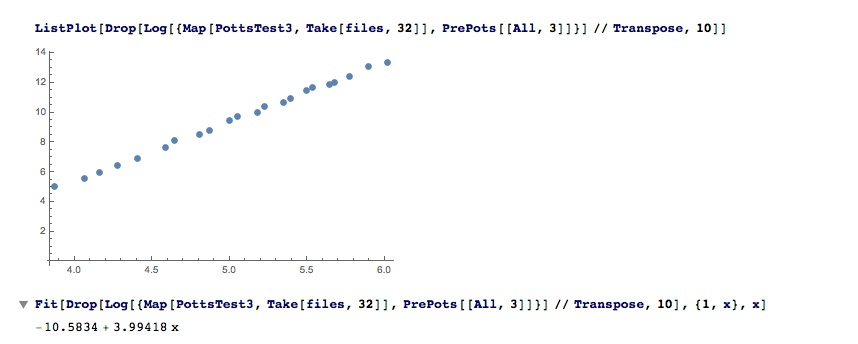
\includegraphics[scale=.4]{runtime.jpeg} % requires the graphicx package
\end{figure}

}

%%%%%%%%%%%%%%%%%%%%%%%%%

\frame
{
\frametitle{Computation}
This algorithm illustrates the issue of large constants in polynomial time algorithms, as using the loops, this would probably take several hundred years for several thousand points.  HOWEVER, it is a massively parallel problem.  Using matrix multiplication reduces the runtime by at least an order of 100 (strictly from parallelization, since these are generally not sparse matrices and I don't think there is any good fast matrix multiplication implemented in my code.) Memory then becomes a problem. \begin{remark}Implement and optimize this code in as a open parallel program, with good numerical error tracking.  Build a database of discrepancies.\end{remark}
}

%%%%%%%%%%%%%%%%%%%%%%%%%
\frame
{
\frametitle{Computation}
This algorithm also allows optimization to find minimal discrepancy point sets, but it is horrible since it depends on the partitions of $N$. So for a simplex, it is nice.  Four points on $\mathbb{S}^2$ can be optimized by hand (almost).  
Under various assumptions, the minimum configuration and associated cap $C$ allows one to pass support points across the boundary by symmetry. Then at the minimum discrepancy configuration
\[
 |\operatorname{Vol}(C) - 1/4 | = |1-\operatorname{Vol}(C)| \implies \operatorname{Vol}(C)= 5/8,  \operatorname{D}(X_N) \ge 3/8.
\]
This is attained at configurations that do not correspond to the regular simplex.  Then the 2-point discrepancy comes into play.% A similar argument indicates that the minimal discrepancy of a simplex is asymptotic to 1/2 in dimension.
%\begin{remark}Do this better for larger point sets.\end{remark}

}

%%%%%%%%%


\frame
{
\frametitle{Computation}
Numerical minimization hinted at $.375 = 3/8$ and can be symbolically solved to give discrepancies of

$$\frac{512+19 \sqrt{466-38 \sqrt{105}}+\sqrt{210
   \left(233-19 \sqrt{105}\right)}}{2048} = \frac{3}{8}
$$

$$\frac{1024-19 \sqrt{466-38 \sqrt{105}}-\sqrt{210
   \left(233-19 \sqrt{105}\right)}}{2048} = \frac{3}{8}$$
  }\frame
{
\frametitle{Computation} 
   \begin{figure}[htbp]
      \centering
      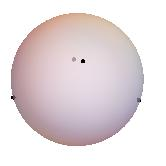
\includegraphics[scale=.5]{tetpoints.jpg} % requires the graphicx package

   \end{figure}
  }\frame
{
\frametitle{Computation} 
      \begin{figure}[htbp]
      \centering
      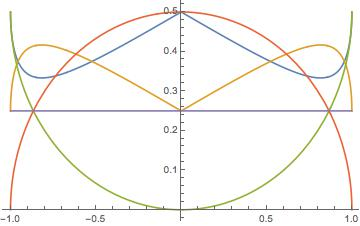
\includegraphics[scale=.5]{discrepancygraph.jpg} % requires the graphicx package

   \end{figure}
}

%%%%%%

%%%%%%%%%% graph of the discrepancies
%\frame
%{
%\frametitle{Discrepancy}
%\begin{figure}[htbp]
%   \centering
%   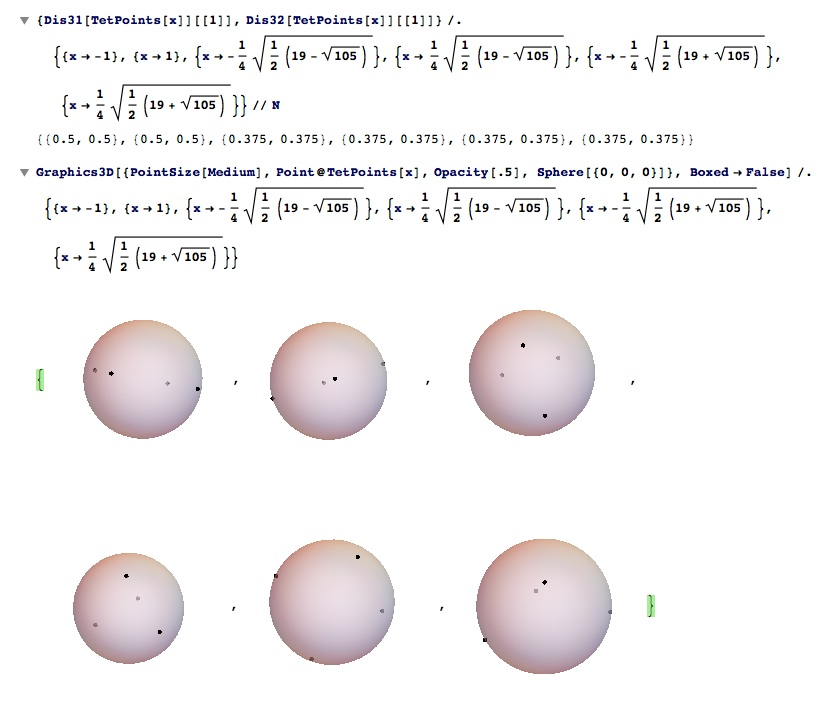
\includegraphics[scale=.2]{optsimp.jpeg} % requires the graphicx package
%\end{figure}
%
%}


%%%%%%%%%%
\frame
{
\frametitle{Discrepancy}
\begin{figure}[htbp]
   \centering
   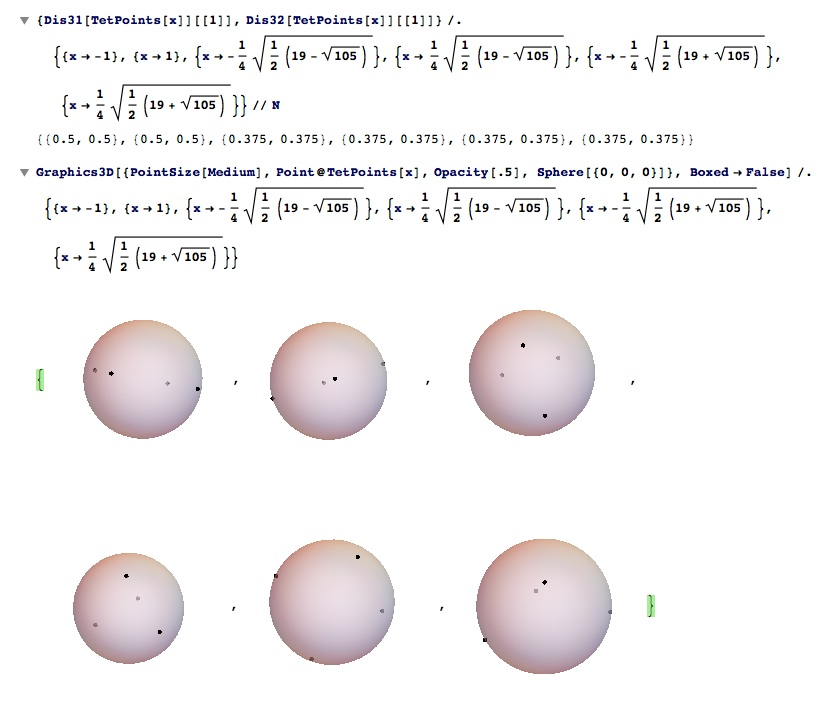
\includegraphics[scale=.2]{optsimp.jpeg} % requires the graphicx package
\end{figure}

}

%%%%%%%%%%%%%%%%%%%%%%%%%
\frame
{
\frametitle{Variance}
One last remark is that the variance

\[
\operatorname{Var}_C[X_N] = \int_{\mathbb{S}^{d}} \operatorname{D}_C^2 \,\mathrm{d} \sigma.
\]

is a quantity that we are actively investigating but is perhaps currently both fuzzy and technical.  There are some nice ways to look at it as a quality of measures parametrized by the radius of the cap size and the function spaces.  It also seems to fit well with a statistical mechanical property of point processes (the hyperuniformity) and their behavior in the thermodynamic limit.\begin{remark}Understand these quantities from multiple perspectives (integral geometry, measure theory, optimal transport, statistical mechanics, discrete/combinatorial geometry).\end{remark}
}

%%%%%%%%%%%%%%%%%%%%%%%%%

\end{document}
